\documentclass[arbeit=studie, oneside, BCOR=12mm]{ArbeitRST}
% Die Option BCOR legt den Rand für die Bindekorrektur links fest
% (verschiebt das ganze Dokument nach rechts auf dem Papier, damit
% Platz zum Binden ist
\usepackage{enumitem}
\usepackage{graphicx}
\usepackage{float}
% bib-Datei mit den Literaturangaben
% Nutzung von biber/biblatex, Erläuterungen
% siehe Text!
% =========================================
\addbibresource{SA_Rockstroh_Literatur.bib}

% Zwei Parameter zum Verändern des Layouts
% ========================================
% \parindent -> Legt fest, mit welcher Einrückung jeder neue
%               Absatz beginnen soll
% \parskip -> Legt fest, wieviel vertikaler Abstand zwischen zwei
%             Absätzen liegen soll
%
% Tipp: Entweder parindent auf Null und parskip auf einen Wert
% ungleich Null (z.B. 2ex) oder umgekehrt. Beide Werte ungleich
% Null macht satztechnisch keinen Sinn. 1ex = Breite des 
% Buchstabens x
\setlength{\parindent}{0ex}
\setlength{\parskip}{2ex}


% Einige Einstellungen für das hyperref-Paket
% =========================================== 
% Hiermit können Links, Gleichungsnummern etc. farbig dargestellt
% werden was die Navigation im elektronischen Dokument vereinfacht. An
% dieser Stelle können Sie die Farbgebung anpassen. Druckversion bitte
% ohne farbige Links erstellen, siehe Option unten!
\hypersetup{
    unicode=false,          % non-Latin characters in Acrobat’s bookmarks
    pdftoolbar=true,        % show Acrobat’s toolbar?
    pdfmenubar=true,        % show Acrobat’s menu?
    pdffitwindow=false,     % window fit to page when opened
    pdfstartview={FitH},    % fits the width of the page to the window
    pdftitle={RST Vorlage}, % title
    pdfauthor={Author},     % author
    pdfsubject={Subject},   % subject of the document
    pdfcreator={Creator},   % creator of the document
    pdfproducer={Producer}, % producer of the document
    pdfkeywords={keyword1} {key2} {key3}, % list of keywords
    pdfnewwindow=true,      % links in new window
    colorlinks=true,        % false: boxed links; true: colored links
    linkcolor=blue,         % color of internal links (change box color with linkbordercolor)
    citecolor=green,        % color of links to bibliography
    filecolor=magenta,      % color of file links
    urlcolor=cyan           % color of external links
}

% Entfernt die farbigen Markierungen - bitte Druckversion mit dieser Option kompilieren
%\hypersetup{hidelinks}



% =================================================================
\begin{document}

% Titelseite
% ==========

% Name des Verfassers
\author{Jonathan Rockstroh}

% Geburtsort
\geburtsort{Pirna}

% Geburtsdatum
\geburtsdatum{14. Mai 1997}

% Titel der Arbeit
\title{Semantische Katalogisierung und formale Repräsentation regelungstechnischer Systemmodelle}

% Untertitel
%\subtitle{}

% Angabe der Betreuer
\betreuer{Dr.-Ing. C. Knoll}

% Datum der Einreichung
%\date{2. Februar 2222}


% Zunächst für das Vorgeplänkel römische Seitenzahlen und einfacher Seitenstil
% ============================================================================
\pagenumbering{Roman}
\pagestyle{plain}


% Titelseite erstellen
\maketitle


% Selbstständigkeitserklärung
% ===========================

% Ort der Selbstständigkeitserklärung (Standard: Dresden)
\selbstort{Pirna}

% Datum der Selbstständigkeitserklärung (Standard: aktuelles Systemdatum)
\selbstdatum{1. September 2021}

% Selbstständigkeitserklärung erstellen
\selbststaendigkeitserklaerung


% Kurzfassung / Abstract
% ======================
\kurzfassung{An dieser Stelle fügen Sie bitte eine deutsche Kurzfassung ein.}{Please insert the English abstract here.}


% Inhaltsverzeichnis
% ==================
\tableofcontents

% Ggf. Symbolverzeichnis
% ======================
\chapter*{Verzeichnis der Abkürzungen \markboth{VERZEICHNIS DER ABKÜRZUNGEN}{}} \label{ch:Symbolverzeichnis}
\addcontentsline{toc}{chapter}{Verzeichnis der Abkürzungen}
\begin{tabular}{ll}
	YAML & Yet Another Markup Language \\
	OCSE & Ontology of Control System Engineering \\
	ACKRep & Automation and Control Knowledge Repository \\
	KS & Klassifikationssystem \\
	IB & Informationsblock \\
	DGL & Differentialgleichung \\
	DAE & Differential Algebraic Equation (dt. Differential-Algebraische Gleichung) \\
	PDE & Partial Differential Equation (dt. Partielle Differentialgleichung)
\end{tabular}

% Ggf. Abbildungsverzeichnis
% ==========================
\listoffigures


% Ggf. Tabellenverzeichnis
% ========================
\listoftables


% ========================
% Beginn Inhalt der Arbeit
% ========================

% Ab hier arabische Seitenzählung und heading Seitenstil
\pagestyle{scrheadings}
\pagenumbering{arabic}

% Kap 1: Einleitung | Letzter Schritt beim Ausarbeiten
% Hauptteil
%	Zusammenstellung von Grundlagen -> VL, verwendete Methoden, Stand der Technik, Ist-Stand, theoret. Grundlagen
%	- Übersicht zu bestehenden Modellübersichten/-katalogen + Bewertung
%	Vorgehensweise, neue Fragen, Zwischenergebnisse
%	- Ziel/ was wünschenswert, Anwendungsintention
%	- Ausarbeitung: bestehendes wissen + Abstrahierung von Eigenschaften
%	- Diskussionen bzgl KS
%	Ergebnisse
%		Katalog - Aufbau --> Übersichtsansicht ähnlich zu ACKRep
%		Einordnug, Bewertung, Selbstkritik - was kann es, was kanns nicht und was für Änderung notwendig
% Finales Kap: Zusammenfassung und Ausblick
%	- Zusammenfassung des Kataloges/Übesichtserstellung -> Inhalt des Kataloges als Übersicht ausgeben

% Kapitel 1: Einleitung
% 1.1 Motivation
% 1.2 Präzisierung der Aufgabenstellung --> Katalog, KS, Modellrepräsentation - Text + Code
\chapter{Einleitung}
\label{Ch:Einleitung}
%\section{Motivation}
%\label{Ch:Einleitung:Sec:Motivation}
% Inhalt: Kurze Erklärung warum ein Katalog von Modellen sinnvoll ist und was die Idee attraktiv macht.

Die Regelungstechnik befasst sich mit der gezielten Beeinflussung und Analyse von regelungstechnischen Systemen. Dies geschieht mithilfe regelungstechnischer Systemmodelle, welche mittels Methoden der Modellbildung erstellt werden. Diese werden in der Literatur verwendet, um ausgewählte Problemstellungen (z.\,B. Regler- oder Beobachterentwurf) mittels regelungstechnischer Methoden zu lösen. Dabei ist die Kenntnis eines ausgewählten Teils der Modelleigenschaften wichtig, da bestimmte Methoden nur anwendbar sind, wenn bestimmte Modelleigenschaften (z.\,B. Steuerbarkeit oder Linearität) vorhanden sind. Ebenso nutzen manche Methoden bestimmte Modelleigenschaften, wie Flachheit oder Passivität, für die Problemlösung aus. Die erzielte Lösung wird aktuell praktisch immer mithilfe computergestützter Simulationen getestet und bewertet.

Die Systemmodelle sind also ein sehr wichtiger Bestandteil der Regelungstechnik. Die Recherche und Verwendung (z.\,B. für Analysen oder Simulationen) von Systemmodellen, erfordert aktuell jedoch oft ein nicht unerhebliches Zeitinvestment. Unter anderem aufgrund einer uneinheitlichen (mathematischen) Darstellung und der so gut wie nie vorkommenden Veröffentlichung von Quellcode. Diese Thematik wird in \autoref{Ch:Vorbetrachtung:Sec:CurrentState} ausführlicher betrachtet. \\
Die Kenntnis der Modelleigenschaften ist sowohl für die Lösung regelungstechnischer Problemstellungen, als auch für die Untersuchung von Modellen auf ebendiese Eigenschaften wichtig. Ebenso ist es wichtig, dass bekannte Modelleigenschaften, zumindest innerhalb des Fachbereiches, einheitlich benannt werden. So wird eine, in Bezug auf die Begriffsbedeutung, eindeutige Kommunikation gewährleistet. 

\section{Präzisierung der Aufgabenstellung}
Um die Situation in Bezug auf die Recherche und Repräsentation von Systemmodellen zu verbessern, wird in dieser Arbeit ein Katalog regelungstechnischer Modelle entworfen. Er soll diese zentral erfassen und einheitlich repräsentiert zur Verfügung stellen. Die Modelleigenschaften sollen, einer einheitlichen Namensgebung folgend, im Katalog erfasst werden. Die einheitliche Namensgebung dieser soll durch ein Klassifikationssystem erreicht werden, welches das Wissen bezüglich regelungstechnischer Modelle gebündelt darstellen soll. Zudem sollen möglichst viele Modelle implementiert werden, um diese für computergestützte Analysen und Simulationen verwendbar zu machen. 




%Inhalt: Aufgabenstellung in stichpunktartigen Sätzen.
%
%Im Rahmen dieser Studienarbeit soll eine Katalog für regelungstechnische Systeme entworfen werden. Darin sollen Modelle als Textrepräsentation und (optional) zusätzlich als implementierter Code enthalten sein. Für beide Repräsentationsarten soll es eine einheitliche Repräsentationsweise geben. Die Umsetzung so erfolgen, das neue Modelle möglichst einfach hinzugefügt werden können. Ebenso soll ein Klassifikationssystem erstellt werden mit dem die Modelle innerhalb der regelungstechnischen Theorie eingeordnet werden können. Das Klassifikationssystem soll auf eine signifikante Anzahl regelungstechnischer Veröffentlichungen angewandt werden. Außerdem sollen ausgewählte  Modelle implementiert werden.
%
%Original (letzter Part): Ziel der Arbeit ist es, mittels sogenannter ontologischer Methoden ein Klassifikationsystem zu erstellen und auf eine signifikante Anzahl (z.B. 50) regelungstechnischer Veröffentlichungen anzuwenden. Zudem sollen die wichtigsten Modelle aus den Veröffentlichungen in Python implementiert und mittels einer Hierarchie semantischer Eigenschaften (z.B. "nichtlinear", "Zustandsdimension: 8", "Flachheitsstatus: nicht flach") erfasst werden.

%--- Noch zu verfassen. ---

% Kapitel 2: (Vor)Überlegungen und Vorgehensweise
\input{SA_Rockstroh_Kap_2_Vorüberlegungen}

% Kapitel 3: Katalog von Modellen der Regelungstechnik
% 3.1 Katalogstruktur
% 3.2 Klassifikationssystem
% 3.2.1 Dateistruktur des Klassifikationssystems
% 3.2.2 Implementierung des Klassifiaktionssystems
% 3.2.3 Metadata-File --> vielleicht auch in Katalogstruktur
% 3.3 Vorlage zur schriftlichen Modelldokumentation
% 3.4 Vorlagen zur Modellimplementierung  
% 3.5 Beispiel anhand einer oder zwei implementierter Modelle
% 3.5.1 Hinzufügen neuer Modelle
% !TeX root = SA_Rockstroh_Main.tex
\chapter{Katalog dynamischer und regelungstechnischer Modelle}
\label{Ch:Ergebnisse}
% Ziel/Inhalt: Nur die Ergebnisse und keine großartigen Begründungen. Die sollen prinzipiell alle im vorherigen Kapitel stehen.
In diesem Kapitel wird der erstellte \textit{Katalog dynamischer und regelungstechnischer Modelle} vorgestellt. Angefangen wird mit der Struktur des Kataloges. Danach werden das Klassifikationssystem(s. \ref{Ch:Ergebnisse:Sec:KS}), die Modelldokumentation(s. \ref{Ch:Ergebnisse:Sec:Dokumentation}) und die Modellimplementation(s. \ref{Ch:Ergebnisse:Sec:Implementation}) als wichtige Elemente des Kataloges beschrieben. Eine Auflistung der aktuell vorhandenen Modelle(s. \ref{Ch:Ergebnisse:Sec:Modelle}) und eine Beschreibung des Ablaufes der Katalogerweiterung(s. \ref{Ch:Ergebnisse:Sec:Erweiterung}) schließen das Kapitel ab.
% Alternative Einführung: Like KS - Beschreibung was der Katalog ist.
% Einschub zur Terminologie: Etwas wird gemacht - ist schon umgesetzt. Etwas soll gemacht werden - noch nicht umgesetzt/praktiziert.
% ===========================================
% ------------- Katalogstruktur -------------
% ===========================================
\section{Katalogstruktur}
\label{Ch:Ergebnisse:Sec:Struktur}
Der Katalog besteht aus folgenden Elementen: Dem \textit{Klassifikationssystem}, dem Python Package \textit{GeneralModel} und Modelleinträgen, die aus einer \textit{Metadaten-Datei}, der \textit{Modelldokumentation}, einer \textit{Parameter-Datei} und, optional, aus der implementierten \textit{Modellklasse}. Für jede Datei eines Modells gibt es eine Vorlage. Die Beziehungen zwischen den Elementen sind in \autoref{fig:Katalogstruktur} dargestellt.

% BILD: Katalogstruktur
% =====================
\begin{figure}[H]
	\centering
	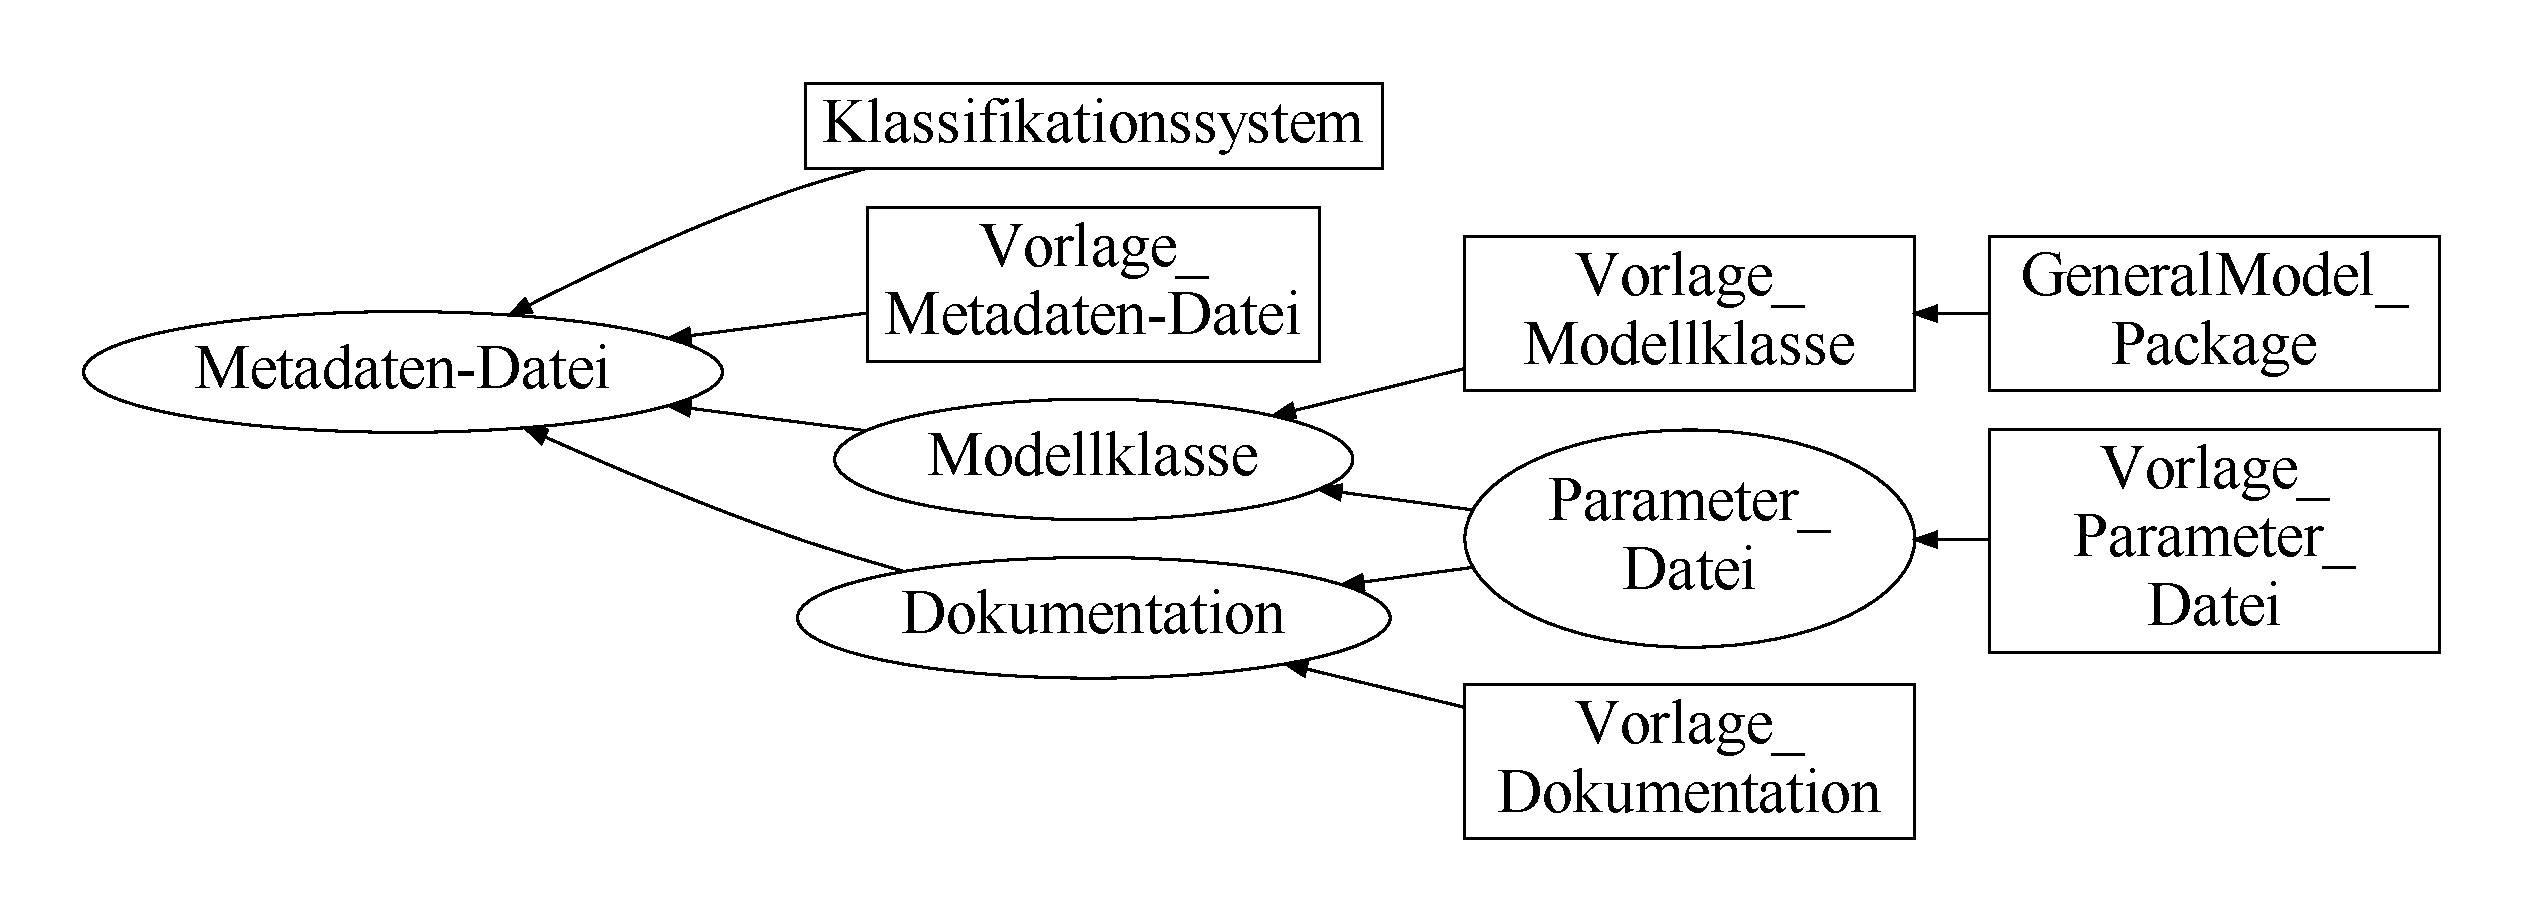
\includegraphics[width=1\linewidth]{Katalogstruktur}
	\caption[Katalogstruktur]{Katalogstruktur. Elemente in Ellipsen existieren individuell für jedes Modell. Elemente in Rechtecken existieren genau ein Mal im Katalog.}
	\label{fig:Katalogstruktur}
\end{figure}
%
Das \textit{Klassifikationssystem} ist eine Übersicht der Modelleigenschaften und deren Beziehungen untereinander. Die Einträge in dem Feld für die Modelleigenschaften in der Metadaten-Datei(\textit{tag\_list}) sind bevorzugt Namen von Kategorieknoten aus dem KS. Es sorgt für eine einheitliche Namensgebung der Modelleigenschaften(s. Anforderung \ref{A.Modelleigenschaften}). 

Das Python Package \textit{GenericModel} stellt die Python Klasse \textit{GenericModel} zur Verfügung von der alle Modellklassen der implementierten Modelle erben. Sie stellt ein Variablen- und Methodenset bereit, das alle Modellklassen gemeinsam haben.

Die \textit{Metadaten-Datei} ist eine Datei im YAML-Format, die Felder für Informationen enthält, in die Informationen des zugehörigen Modells eingetragen werden können. Es gibt Felder für Informationen \dots 
\begin{itemize}[label=$\bullet$]
	\item über das Modell (Modellname, Kurzbeschreibung, Modelleigenschaften, Dateinamen der Modellbilder)
	\item für eine Umsetzung des Kataloges als Datenbank(Key, Predecessor-Key, Implementation-Key)
	\item anderer Art (Modellersteller, Erstellungsdatum, Liste der Bearbeiter, Externe Referenzen)
\end{itemize}
Das Konzept und die Umsetzung der Metadaten-Datei stammt aus dem \textit{ACKRep}\footnote{ACKRep Testinstanz. \tiny{URL}\normalsize: \url{https://testing.ackrep.org/}}. 
% Noch schreiben welche Informationen im aktuellen Stand gegeben werden?

Die \textit{Modelldokumentation} ist die textuelle Notation des Modells. Sie wird im \LaTeX-Format geschrieben. Nach jeder Bearbeitung wird die PDF-Datei aus der \LaTeX-Datei erzeugt. 

Die \textit{Parameter-Datei} ist eine Python-Datei. Diese enthält beispielhafte Parameterwerte für das Modell. Das Ausführen der Datei erzeugt eine Tabelle mit den beispielhaften Parameterwerten im \LaTeX-Format und speichert diese in einer Datei Namens \textit{parameters.tex} im Ordner der Modelldokumentation ab. Außerdem stellt Sie eine Methode für die implementierte Modellklasse bereit, welche die Parameter des Modells als Rückgabewert hat.

Die implementierte \textit{Modellklasse} ist eine Python-Datei, welche das Modell als Python-Klasse enthält. 

Die \textit{Vorlagen} für die Metadaten-Datei, die Parameter-Datei, die Modelldokumentation und -implementation sind Dateien, welche den Arbeitsaufwand für das Anlegen neuer Modelle verringern sollen(siehe Entscheidung \ref{E.Vorlagen}). Die repetitiven Elemente für die entsprechenden Dateien sind in den Vorlagen schon vorhanden, sodass nur die Modellspezifischen Elemente neu geschrieben werden müssen. Die Verwendung der Vorlagen stellt außerdem eine einheitliche Struktur der Dateien sicher.

Die Ordnerstruktur des Kataloges liegt in einem Git-Repositorium\footnote{Der Katalog hat kein eigenes Repository, sondern liegt aktuell im Git-Repository dieser Studienarbeit. Deshalb wird an dieser Stelle kein Link zur Verfügung gestellt.}(s. Entscheidung \ref{E.Git}).  

% =================================================
% ------------- Klassifikationssystem -------------
% =================================================
\section{Klassifikationssystem}
\label{Ch:Ergebnisse:Sec:KS}
Das \textit{Klassifikationssystem (KS)} stellt eine Wissensrepräsentation dar. Es lehnt stark an die in \cite{KNHE20a} eingeführte \textit{OCSE} an, von der es sich insofern unterscheidet, das im KS nur die Teilbereiche des Wissens der Mathematik, Regelungs- und Steuerungstheorie enthalten sind, die sich auf regelungstechnische Systeme und Modelle beziehen. Die im KS verwendeten Bezeichnungen sollen in den Metadaten-Dateien der Modelle bevorzugt verwendet werden. \\
Es ist anzumerken, dass das KS keine vollständige Wissensrepräsentation darstellt. Das liegt daran, dass das darzustellende Wissen sehr umfangreich ist und eine vollständige Darstellung dessen im Rahmen dieser Studienarbeit nicht möglich war. Weiter könnte man auch die Frage stellen, ob überhaupt eine vollständige Darstellung des beabsichtigten Wissensbereiches existiert, da das Wissen dynamisch durch neue Entdeckungen erweitert wird. Diese Diskussion soll hier aber nicht weitergeführt werden. 

Bei einem konkreten Modell im Katalog finden sich die Einträge des KS im Informationsfeld \textit{tag\_list} der Metadaten-Datei wieder. In diesem Informationsfeld werden die Modelleigenschaften und dessen Werte notiert. Für die Einträge in der \textit{tag\_list} gilt eine Open-World Annahme. Wenn eine Eigenschaft nicht in der \textit{tag\_list} enthalten ist, dann enthält der Katalog keine Aussage darüber, ob das Modell die Eigenschaft besitzt oder nicht.

Das KS besteht aktuell aus 90 Knoten. \autoref{fig:KS_AttributesSnippet} zeigt ein Ausschnitt des KS.

% BILD: Ausschnitt KS, aus Modelleigenschaften
% ============================================
\begin{figure}
	\centering
	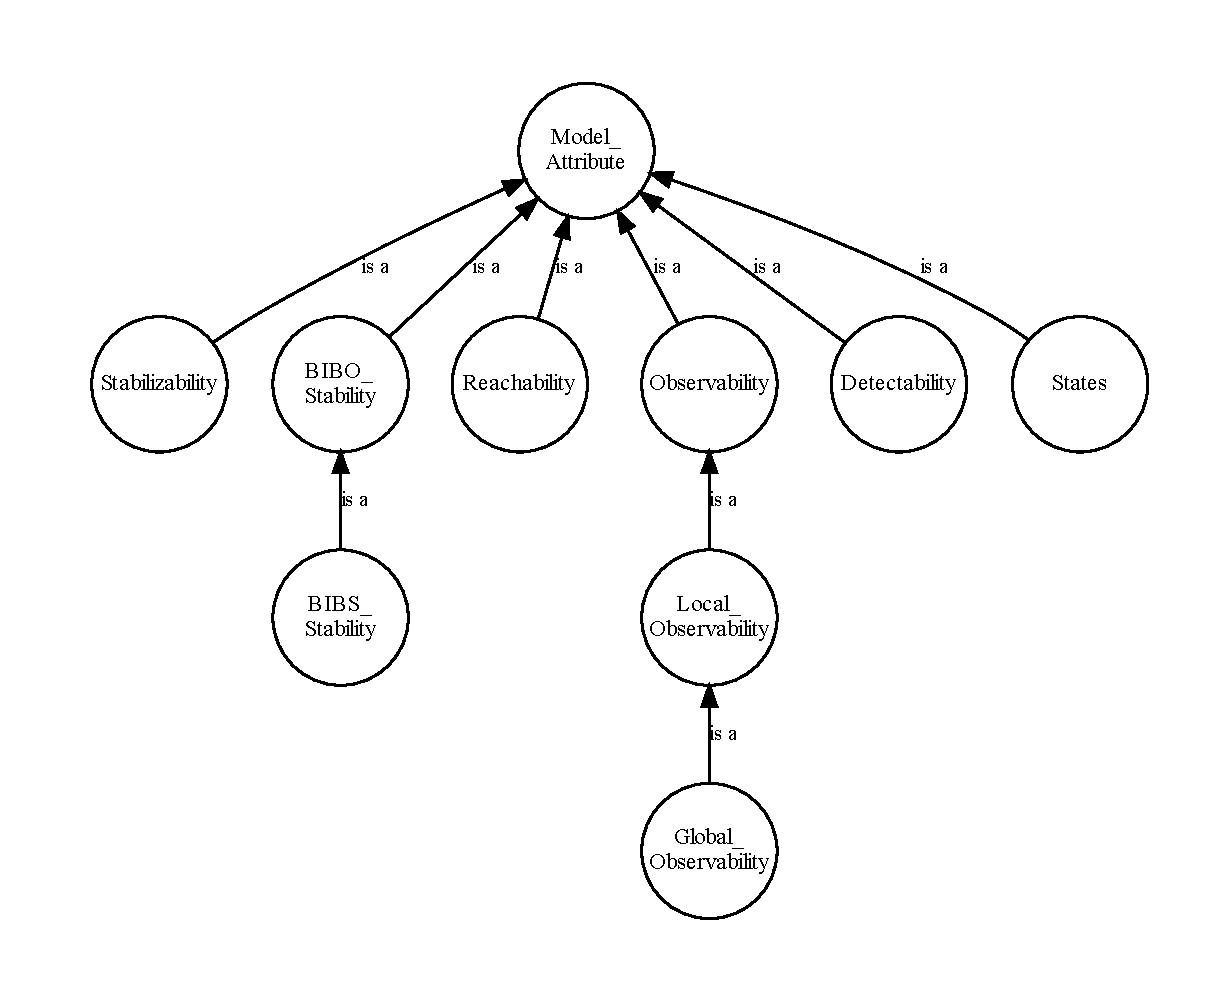
\includegraphics[width=0.9\linewidth]{Ausschnitt_KS_Attributes}
	\caption{Auschnitt des KS aus der Hauptkategorie \textit{Modelleigenschaften}}
	\label{fig:KS_AttributesSnippet}
\end{figure}

% =============================================================
% ------------- Aufbau des Klassifikationssystems -------------
% =============================================================
\subsection{Aufbau des Klassifikationssystems}
\label{Ch:Ergebniss:Sec:KS:SubSec:Aufbau}
Das KS ist ein Semantisches Netz(s. \ref{E.KS_SemantischesNetz}), welches durch einen gerichteten, kreisfreien Graphen repräsentiert wird. Es gibt folgende Knotentypen: Kategorie-, Objekt-, Werte, und Wertetypknoten. 
Die Kanten zeigen Beziehungen zwischen den Knoten des KS auf, die durch die Kantenbeschriftungen spezifiziert werden. Es gibt folgende Kantennamen: \glqq is a\grqq, \glqq Value\grqq, \glqq Type\grqq und \glqq Object\grqq. Der Kantenname kennzeichnet zudem den Knotentyp des Startknotens der Kante. Jeder Endknoten einer Kante ist ein Kategorieknoten. Die Beziehung zwischen Knotentypen und Kantennamen wird in \autoref{table:KS_KantenUndKnoten} gezeigt.
% TABELLE: Kantennamen - Knotentypen Beziehung
% ============================================
\begin{table}[H]
	\centering
	\begin{tabular}{l|c|l}
		Startknotentyp & Kantenname & Endknotentyp \\ \hline
		Kategorieknoten & is a & Kategorieknoten \\
		Werteknoten & Value & Kategorieknoten \\
		Wertetypknoten & Type & Kategorieknoten \\
		Objektknoten & Object & Kategorieknoten
	\end{tabular}
	\caption{Beziehung zwischen Kantennamen und Knotentypen}
	\label{table:KS_KantenUndKnoten}
\end{table}
%
Die Kategorieknoten, außer der Ursprungsknoten und die Knoten der Hauptkategorien, können als Modellattribute interpretiert werden. \\
Die Kategorieknoten im KS werden durch ihren eindeutigen Namen identifiziert(s. \ref{E.KS_Namensgebung}).\\
Jeder Knoten $k$, außer der Ursprungsknoten, ist entlang eines gerichteten Pfades $P(k)$ mit dem Ursprungsknoten verbunden. Wird einem Modell ein Knoten $k_i$ des KS als Modellattribut zugewiesen, dann hat das Modell auch alle Knoten, außer Ursprungs -und Hauptknoten, entlang des gerichteten $P(k_i)$ als Modellattribut. Aus diesem Grund wird in der \textit{tag\_list} der Metadaten-Datei immer nur die spezifischste Eigenschafte eines Pfades angegeben. % Beispiel?

Der Ursprungsknoten \textit{Property\_Of\_Classification\_System} hat die drei Unterkategorien \textit{Property\_Of\_Mathematical\_Representation}, \textit{Model\_Behaviour} und \textit{Usage}. Die Unterkategorien des Ursprungsknoten werden im KS als Hauptkategorien bezeichnet, die jeweils verschiedene Teilmengen von Modellattributen enthalten. Die Hauptkategorien werden wie folgt beschrieben.

\textbf{Eigenschaften der mathematischen Repräsentation}: \\
Umfasst Eigenschaften der mathematischen Repräsentation des Modells.   % ... die aus der math. Rep. direkt hervor gehen. --> Äquivalenzbegriff von Willems

\textbf{Modelleigenschaften}: \\ % Eigenschaften unabhängig von Darstellungsform eines äquivalenten Systems
Umfasst Eigenschaften die aus der mathematischen Repräsentation mit Methoden der Regelungstechnik abgeleitet werden.

\textbf{Verwendung}: \\
Umfasst Aufgabentypen und Anwendungsbereiche in denen die Modelle häufig genutzt werden.

In \autoref{Ch:Vorbetrachtung:Sec:SystemeModelle} wurde erwähnt, dass ein Modell mehrere mathematische Repräsentationen haben kann. Dieser Aspekt führt auf den Begriff der \textit{Äquivalenz} zweier mathematischer Modelle. Zwei mathematische Modelle heißen \textit{Äquivalent}, wenn beide die gleiche Menge an Trajektorien für ihre externen Variablen zulassen\footnote{vgl. \cite{SCH89}, S. 34}. Oder einfacher, wenn beide Modelle das gleiche dynamische Verhalten aufweisen. Das Modell eines Systems kann durch eine Menge äquivalenter mathematischer Modelle repräsentiert werden. Der Unterschied zwischen den Hauptkategorien \textit{Eigenschaft der mathematischen Repräsentation} und \textit{Modelleigenschaften} liegt darin, dass die Elemente eine Menge äquivalenter mathematischer Modelle die gleichen Modelleigenschaften haben, sich aber in ihrer mathematischen Repräsentation unterscheiden.

% ===========================================================================
% ------------- Technische Umsetzung des Klassifikationssystems -------------
% ===========================================================================
\subsection{Technische Umsetzung des Klassifikationssystems}
\label{Ch:Ergebnisse:Sec:KS:SubSec:TechUmsetzung}
Das KS wird technisch durch vier Dateien im YAML-Format realisiert, welche folgende Namen haben: \textit{KS\_Tree\_main}, \textit{KS\_Tree\_Math\_Representation}, \textit{KS\_Tree\_Model\_Attributes} und \textit{KS\_Tree\_Usage}. Die Datei \textit{KS\_Tree\_main} enthält die \textit{Informationsblöcke(IB)} zu dem Ursprungsknoten und den Knoten der Hauptkategorien. Die restlichen drei Dateien enthalten jeweils die Informationsblöcke zu den Knoten der Unterkategorien der Hauptkategorien. \\ 
Ein IB enthält alle Informationen zu genau einem Knoten des KS. Jeder IB in den YAML-Dateien ist ein Mapping. Ein Mapping, gekennzeichnet durch einen Doppelpunkt, setzt einen Schlüssel mit genau einen Wert in Beziehung. Das \textit{dictionary} ist das Python-Äquivalent zu einem Mapping. In jedem IB ist der Name des Knotens der Schlüssel und eine Sequenz ist der Wert. Eine Sequenz ist in YAML eine Folge von Zeilen, die mit einem Strich beginnen und der Inhalt der Zeile stellt einen Eintrag der Sequenz dar. \textit{List} und \textit{tuple} sind die Python-Äquivalente zur Sequenz. Jeder Eintrag der Sequenz steht für ein Attribut des Knotens und ist wiederum ein Mapping, dessen Schlüssel der Attributsname und dessen Wert der Attributswert ist. Die IB\grq s sind durch eine Leerzeile voneinander getrennt. Die Abbildung \ref{fig:IBs} zeigt einige IB\grq s aus der Datei \textit{KS\_Tree\_Math\_Representation}.\\ 
% BILD: Informationsblöcke
%=========================
\begin{figure}[b]
	\centering
	\begin{adjustbox}{padding=15pt 0pt 0pt 0pt, fbox}
	\begin{lstlisting}[basicstyle=\footnotesize]
General_Function:
	- Type: boolean
	- Pre_Node: Property_Of_Mathematical_Representation
	- Edge_Name: is a

DAE: 
	- Type: boolean
	- Pre_Node: General_Function
	- Edge_Name: is a
	\end{lstlisting}
	\end{adjustbox}
	\caption{Informationsblöcke des KS}
	\label{fig:IBs}
\end{figure}

Eine Kante wird durch die Elemente \textit{Pre\_Node} und \textit{Edge\_Name} definiert. Diese stehen jeweils als Einträge in der Sequenz des Informationsblocks des Startknotens der Kante.

Zusätzlich gibt es das Python-Skript \textit{KS\_Create\_Graph}, welches die YAML-Dateien mit Hilfe des Packages \textit{pyyaml}\footnote{Pyyaml-Package: \url{https://pyyaml.org/wiki/PyYAMLDocumentation}} einliest. Zudem erzeugt es einen gerichteten Graphen des Python-Packages \textit{networkx}\footnote{Networkx Package: \url{https://networkx.org/documentation/stable/index.html}} und zeichnet den Subgraphen, der nur die Kategorieknoten enthält mit dem Python-Package \textit{nxv}\footnote{Nxv-Package: \url{https://nxv.readthedocs.io/en/latest/index.html}} in eine Bilddatei.

Ein gerichteter Graph des networkx-Packages besteht aus einer Menge von Knoten und Kanten. Zu jedem Knoten und jeder Kante kann eine beliebig große Menge individuell benannter Attribute hinzugefügt werden. So werden z.\,B. die Kantennamen der entsprechenden Kante als Attribut hinzugefügt. Die Wertetypknoten sind als Attribut eines Kategorieknotens implementiert. Diese Umsetzung des implementierten Graphen ist aus technischer Sicht sinnvoll, da die Information über die Attribute eines Knotens so intuitiver zu erreichen sind. Es soll hier jedoch erwähnt werden, das diese Implementierung von einer korrekten Darstellung des KS als Semantisches Netz abweicht, da Kategorieknoten nur explizit als Knoten aufgeführte Attribute besitzen. Für eine formal korrekte Implementierung des KS als Semantisches Netz müssten Knoten welche die Attribute einer Kategorie darstellen auch explizit als Knoten angelegt werden.\\
Die gewählte Implementierung des KS ist einfach erweiterbar und bearbeitbar. Eine Veränderung im Umfang des KS, also das Hinzufügen neuer Knoten zum KS oder das entfernen von Knoten aus dem KS, wird in der Implementierung durch schreiben neuer IB\grq s oder entfernen bestehender IB\grq s erreicht. Sollen neue Knotentypen zum KS hinzugefügt werden z.\,B. Referenzknoten, welche eine Referenz zur Definition der Kategorie enthalten würden, so werden diese als neuer Eintrag zu den Sequenzen der IB\grq s hinzugefügt.

%TODO: Vllt eher in Ausblick?
Die Implementierung des KS ist auch relativ einfach für eine potenzielle Integration einer Suchfunktion zu öffnen, indem zu dem Python-Skript \textit{KS\_Create\_Graph} eine Methode hinzugefügt wird, welche die networkx-Graphen des KS als Rückgabewert liefert.  
% Networkx-Graphen vom Funktionsumfang potenziell als vollständige maschinelle lesbare Repräsentation des KS und dessen Anwendungen auf die Modelle verwendbar

% ===============================================
% ------------- Modelldokumentation -------------
% ===============================================
\section{Modelldokumentation}
\label{Ch:Ergebnisse:Sec:Dokumentation}
Die Modelldokumentation enthält die textuelle Notation des Modells in einer Datei im \LaTeX-Format. Die Dokumentation besteht aus den Abschnitten: \textit{Nomenklatur}, \textit{Modellgleichungen}, \textit{Herleitung und Erklärungen} und \textit{Referenzen}. Der Abschnitt \textit{Herleitung und Erklärung} ist optional.

\textbf{Nomenklatur}:\\
Die Nomenklatur enthält alle in der Dokumentation genutzten Variablen und eine Beschreibung, für welche Größen diese stehen. Die Nomenklatur ist aufgeteilt in die Sektionen \textit{Nomenklatur für die Modellgleichungen} und \textit{Nomenklatur für die Herleitung}. Die Nomenklatur für die Modellgleichungen enthält die Variablen, die im gleichnamigen Abschnitt verwendet werden und muss in jeder Dokumentation enthalten sein. Die Nomenklatur für die Herleitung enthält alle Variablen die für den Abschnitt \textit{Herleitung und Erklärung} genutzt werden, bis auf die Variablen die in der Sektion \textit{Nomenklatur für die Modellgleichungen} schon enthalten sind. Die Nomenklatur für die Herleitung ist nur zu schreiben, wenn der Abschnitt \textit{Herleitung und Erklärung} existiert.

% BILD: Dokumentation Nomenklatur
% ===============================
\begin{figure}[H]
	\centering
	\fbox{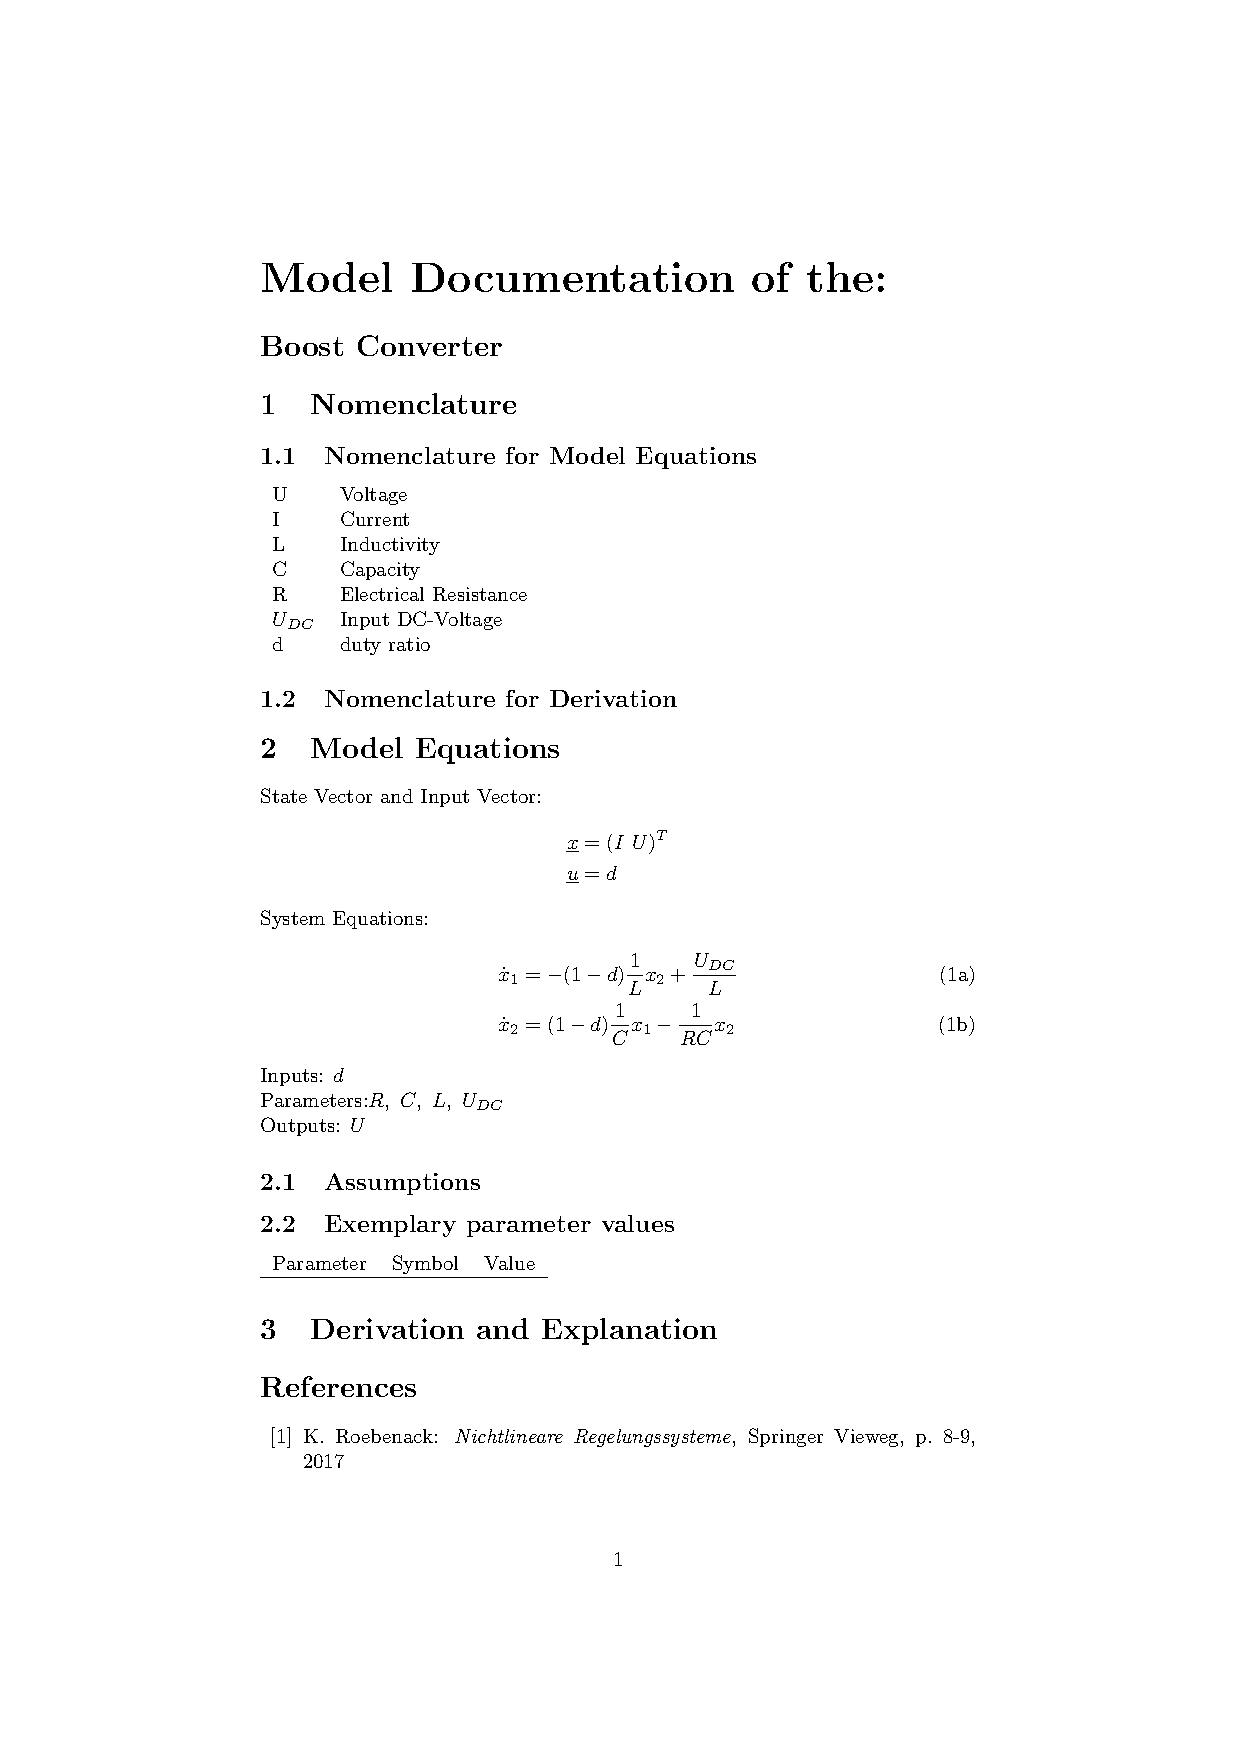
\includegraphics[trim=120 520 120 110, clip, width=0.9\linewidth]{Boost_Converter_Documentation}}
	\caption{Nomenklatur aus der Dokumentation zum Hochsetzsteller (Boost-Converter)}
	\label{fig:BspDok_Nomenclature}
\end{figure}
%
\textbf{Modellgleichungen}:\\
Der Abschnitt \textit{Modellgleichungen} besteht aus einer formalisierten Darstellung der Modellgleichungen und weiteren Sektionen, die gleich noch benannt werden. Die formalisierte Darstellung der Modellgleichungen besteht aus drei Teilen:  
\begin{itemize}[label=$\bullet$]
	\item einer Zuordnung der Variablen zum generalisierten Zustands-, Eingangs- und (optional) Ausgangsvektor
	\item einem Gleichungssystem von Differentialgleichungen erster Ordnung(s. \ref{E.Textdok}), das die generalisierten Zustands- und Eingangsvariablen verwendet
	\item der Benennung, welche Variablen Parameter sind
\end{itemize} 

% BILD: Dokumentation Modellgleichungen
% =====================================
\begin{figure}[h]
	\centering
	\fbox{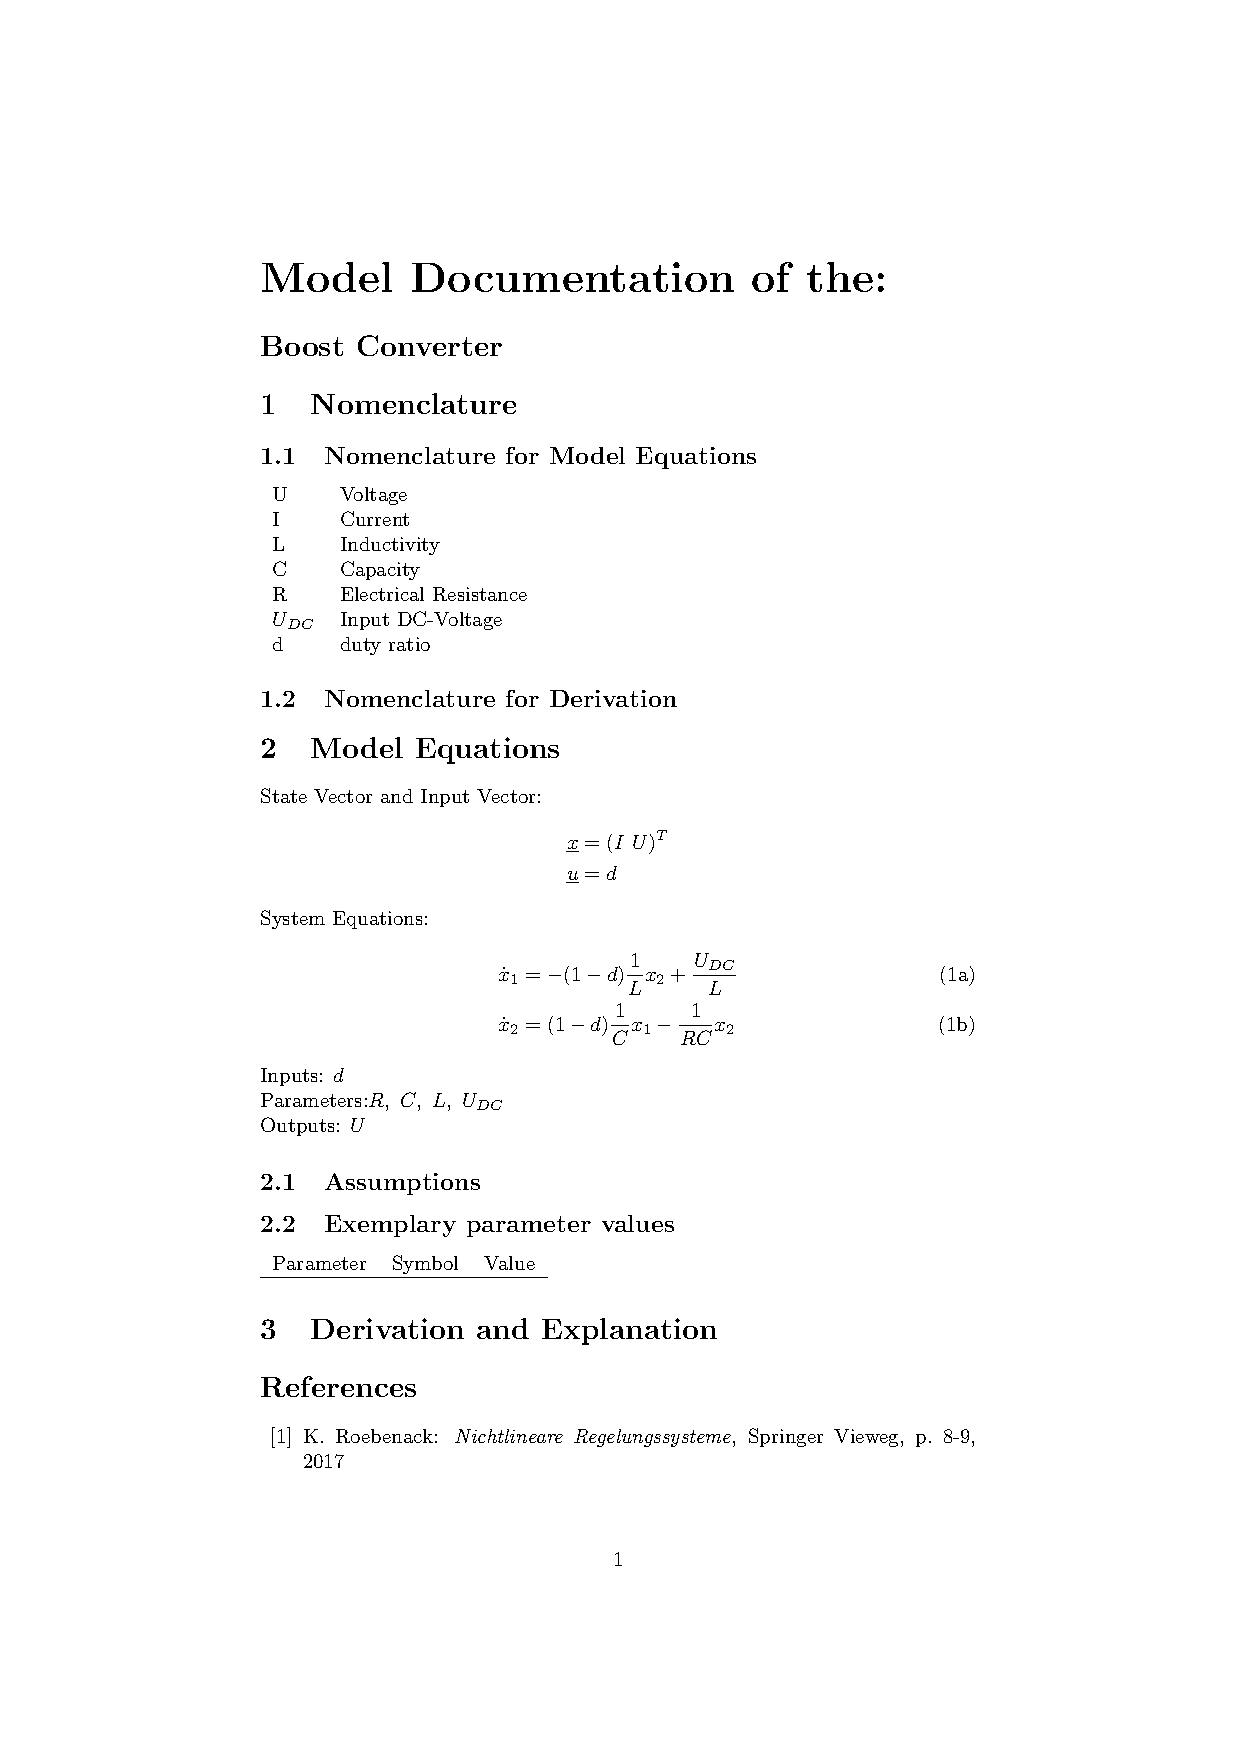
\includegraphics[trim=120 300 120 340, clip, width=0.9\linewidth]{Boost_Converter_Documentation}}
	\caption{Gleichungen aus der Dokumentation zum Hochsetzsteller (Boost-Converter)\protect\footnotemark}
	\label{fig:BspDok_ModelEquations}
\end{figure}
\footnotetext{Modell stammt aus \cite{ROEB17} Abschnitt 1.3}
%
Die weiteren Sektionen sind recht frei gestaltbar und sollen weitere nützliche Informationen zu dem Modell liefern. Aktuell sind in der Vorlage nur die Sektionen \textit{Annahmen} und \textit{Beispielhafte Parameterwerte} explizit formuliert. Weitere Sektionen können vom Ersteller des Modells nach eigener, subjektiver Einschätzung der Sinnhaftigkeit hinzugefügt werden. Denkbar wäre, angenommen es handelt sich um ein flaches Modell, z.\,B. ein Abschnitt der flache Ausgänge angibt. Die Sektion \textit{Beispielhafte Parameterwerte} ist als einzige unter den weiteren Sektionen zwingend zu füllen. Dies geschieht mehr oder weniger automatisch, da die Datei \textit{paramters.tex}, die durch die \textit{Parameter-Datei} erstellt wird, dafür eingebunden wird.

\textbf{Herleitung und Erklärungen}:\\
Dieser Abschnitt ist für die Dokumentation optional. Er soll die Möglichkeit bieten die Herleitung des Modells zu beschreiben oder weitere aus Sicht des Modellerstellers sinnvolle Erklärungen zu liefern.

\textbf{Referenzen}:\\
Enthält die Referenzen, die für die Erstellung der Modelldokumentation verwendet wurden.

Aus der \LaTeX-Datei der Modelldokumentation wird eine für Menschen gut lesbare PDF-Datei erzeugt. 

% =================================================
% ------------- Modellimplementation  -------------
% =================================================
\section{Modellimplementation}
\label{Ch:Ergebnisse:Sec:Implementation}
Modelle des Kataloges werden in Form einer Python-Klasse implementiert. Bei Initialisierung eines Objektes der Modellklasse können dem Konstruktor die Zustandsdimension, eine Eingangsfunktion und ein Parametervektor übergeben werden. Alle diese Variablen haben Standardwerte. Jede Modellklasse bezieht ein Standardset von Parameterwerten aus der \textit{Parameter-Datei} (die Standardparameter sind also identisch mit den beispielhaften Parameterwerten aus der Dokumentation) und hat eine Standardfunktion für die Modelleingänge bzw. die Eingangsfunktion integriert.\\ 
Ein Modell kann also einfach über ein selbst erstelltes Python-Skript simuliert werden(vgl. \ref{A.Implementierung}), indem eine Objekt der Modellklasse erzeugt wird, ein Startvektor für den Modellzustand definiert wird und anschließend das Modell mit einer geeigneten Methode(z.\,B. \textit{solve\_ivp} des Python-Packages \textit{scipy}\footnote{SciPy-Package: \url{https://www.scipy.org/}}) simuliert wird. Die Methode \textit{get\_rhs\_func}\footnote{\textit{rhs} steht für \textit{right hand side}} der Modellklasse stellt die dafür benötigte Python-Funktion zur Verfügung.

Die Parameter und die Eingangsfunktion eines Modellobjektes können nach Initialisierung mit den Methoden \textit{set\_parameters} und \textit{set\_input\_func} geändert werden. Die Zustandsdimension ist nur bei Initialisierung einstellbar und das auch nur bei Modellen, deren Zustandsdimension nicht festgelegt ist(z.\,B. beim N-Fach-Integrator).\\
Die Methode \textit{get\_rhs\_symbolic} liefert die symbolischen Modellgleichungen als Rückgabewert. Zur Implementierung der symbolischen Gleichungen wird das Python-Package \textit{sympy}\footnote{SymPy-Package: \url{https://www.sympy.org/en/index.html}} verwendet.

%Obsoloter Absatz?
Jede Modellklasse erbt von der Klasse \textit{GenericModel}, welche eine Menge von Methoden und Variablen definiert, die jede Modellklasse haben muss. Die Methoden, die nicht für jede individuelle Modellklasse angepasst werden müssen sind in der Klasse \textit{GenericModel} bereits implementiert.\\
Innerhalb einer Modellklasse sind nur die symbolischen Gleichungen als Code geschrieben. Die Umwandlung in die numerische Form erfolgt in der Methode \textit{get\_rhs\_func} mit der Methode \textit{lambdify} des Sympy-Packages.
% Hinweis das bei Codesyntax versucht wurde nach PEP8 zu arbeiten?

Mittels der aktuellen Vorlagen können nur Modelle, deren Verhalten durch ein gewöhnliches Differentialgleichungssystem erster Ordnung beschrieben wird, implementiert werden.

% ==============================================
% ------------- Vorhandene Modelle -------------
% ==============================================
\section{Vorhandene Modelle}
\label{Ch:Ergebnisse:Sec:Modelle}
Die aktuell im Katalog enthaltenden Modelle sind in \autoref{table:AktuelleModelle} aufgelistet. 

% TABELLE: Aktuelle Modelle
% =========================
\begin{table}[H]
	\begin{tabular}{r|c|c|c}
		Nr & Name & Modelldimension & Implementiert? \\ \hline
		1 & Hochsetzsteller & 2 & Nein \\
		2 & Brockett-Integrator & 3 & Ja \\
		3 & DC-DC Tiefsetzsteller & 2 & Nein \\
		4 & Heisenberg-Flugrad & 3 & Nein \\
		5 & Kapitzas Pendel & 2 & Ja \\
		6 & Lorenz Attraktor & 3 & Ja \\
		7 & MMC\tablefootnote{Modular Multilevel Converter} & 8 & Nein \\
		8 & N-Fach Integrator & n & Ja \\
		9 & PVTOL mit 2 Kräften\tablefootnote{Planar Vertical Takeoff and Landing [Vehicle] (dt. Senkrechtstarter)} & 6 & Ja \\
		10 & Rössler Attrkator 1979a & 3 & Ja
	\end{tabular}
	\caption{Modelle des Kataloges}
	\label{table:AktuelleModelle}
\end{table} 

% ==============================================
% ------------- Katalogerweiterung -------------
% ==============================================
\section{Katalogerweiterung}
\label{Ch:Ergebnisse:Sec:Erweiterung}
Die letzte Anforderung an den Katalog war, das dieser erweiterbar sein soll (Anforderung \ref{A.Erweiterbarkeit}). In diesem Abschnitt wird beschrieben, welche Schritte für die Erweiterung des Kataloges nötig sind. 

Der Katalog wird über das Hinzufügen neuer Modelle erweitert.

Wir treffen folgende Annahmen:
\begin{enumerate}
	\item Die Recherche für das hinzuzufügende Modell ist abgeschlossen. Die nötigen Informationen zu dem Modell wie Modellgleichungen, beispielhafte Parameterwerte, Beschreibung der Variablen und die dazugehörigen Referenzen sind also schon bekannt.
	\item Der Modellersteller hat sich mit der Ordnerstruktur des Kataloges vertraut gemacht.
\end{enumerate}

Für das Anlegen eines neuen Modells im Katalog sind folgende Schritte notwendig:
\begin{enumerate}
	\item Git installieren und das Git-Repositorium(siehe \ref{E.Git}) des Kataloges herunterladen um eine lokale Kopie des Kataloges und der Vorlagen(siehe Abschnitt \ref{Ch:Ergebnisse:Sec:Struktur} \nameref{Ch:Ergebnisse:Sec:Struktur}) zu erhalten.
	\item Anlegen und benennen eines neuen Modell- und Implementationsordners.
	\item Erstellen der \textit{Metadaten-Datei} im Modellordner mithilfe der Vorlage und Umbenennung dieser in \textit{metadata.yml}.
	\item Erstellen der \textit{Modelldokumentation} im Modellordner mithilfe der Vorlage.
	\begin{enumerate}[label=\textbf{Anmerkung \arabic*}:, wide=0pt, leftmargin=*]
		\item Die Vorlage stellt aktuell nur eine einheitliche Notation für gewöhnliche Differentialgleichungssysteme erster Ordnung zur Verfügung. Modelle, deren Modellgleichungen in ein gewöhnliches Differentialgleichungssystem erster Ordnung transformierbar sind, müssen in ein solches transformiert werden.
		\item Für Modell, deren Modellgleichungen nicht in ein gewöhnliches Differentialgleichungssystem erster Ordnung transformierbar sind, gibt es noch keine festgelegte Notationsvorgabe.
	\end{enumerate}
	\item Erstellen der \textit{Parameter-Datei} im Implementationsordner mithilfe der Vorlage und ausführen\footnote{Zur Erinnerung: Die Parameter-Datei ist ein Python Skript.} dieser.
	\item Die PDF-Datei der Modelldokumentation erzeugen.
	\item (optional, siehe \ref{E.ImplementierungOptional}) Erstellen der \textit{Modellklasse} im Implementationsordner mithilfe der Vorlage.
	\begin{itemize}[label=\textbf{Anmerkung}:, wide=0pt, leftmargin=*]
		\item Aktuell können nur Modelle, die durch ein gewöhnliches Differentialgleichungssystem erster Ordnung beschrieben werden, mithilfe der Vorlage implementiert werden.
	\end{itemize}
	\item Pull-Request ausführen.
\end{enumerate}







% Kapitel 4: Zusammenfassung und Ausblick
% 4.1 Übersicht zu aktuellem Funktions- und Modellumfang
% 4.2 Ausblick
\chapter{Zusammenfassung und Ausblick}
\label{Ch:ZsmfsgAusblick}
\section{Zusammenfassung}
\label{Ch:ZsmfsgAusblick:Sec:Zsmfsg} 
In dieser Studienarbeit wurde die Erstellung eines Kataloges von regelungstechnischen Systemmodellen beschrieben. Angefangen wurde in \autoref{Ch:Vorbetrachtung} mit einer Betrachtung der aktuellen Situation bezüglich der Suche und Implementation von Modellen mit dem Ergebnis, dass diese nicht optimal ist. Außerdem wurden zwei aktuell vorhandene Modellsammlungen beschrieben. 

Danach wurden im \autoref{Ch:Vorbetrachtung:Sec:Anforderungen} zuerst Anforderungen formuliert, die der Katalog haben soll und anschließend eine Reihe von Entscheidungen ausgeführt, die der Erfüllung dieser Anforderungen dienen sollen. Im \autoref{Ch:Vorbetrachtung:Sec:KS} wurden Entscheidungen vorgestellt, die aufgetretene Frage- und Problemstellungen beantworten.

In \autoref{Ch:Ergebnisse} wurde der \textit{Katalog dynamischer und regelungstechnischer Modelle} vorgestellt. Zuerst wurde beschrieben, aus welchen Elementen sich dieser zusammensetzt und wie diese zusammenhängen. Anschließend wurden die Elemente des Kataloges detaillierter betrachtet. Die letzten zwei Abschnitte lieferten eine Übersicht zu den aktuell vorhandenen Modellen und dem vorgehen zum Hinzufügen neuer Modelle.

Der Katalog enthält aktuell nur einen recht kleinen Umfang an Modellen und ist momentan nur für Modelle, die durch gewöhnliche Differentialgleichungen erster Ordnung beschrieben werden ausgelegt und durchdacht worden. Für diese Modelle wurde eine einheitliche Dokumentationsform sowie eine einfach anwendbare Implementationsweise durch die Python-Klasse \textit{GenericModel} entwickelt. Zudem wurde mit der \textit{Metadaten-Datei} eine Schnittstelle hinzugefügt, die es erlaubt, aus dem Katalog eine Datenbank inklusive Suchfunktion zu erstellen. 

Es wurde das \textit{Klassifikationssystem} vorgestellt, welches als Wissensrepräsentation für die Teilbereiche der Mathematik und Regelungstheorie, die sich auf Modelle beziehen, gedacht ist. Es enthält die möglichen Eigenschaften der Modelle und stellt deren Beziehung zueinander dar. Das abgebildete Wissen des Klassifikationssystems enthält die geläufigsten Modelleigenschaften und hat noch viel Erweiterungspotenzial. Es wurde die technische Umsetzung des KS beschrieben, die eine einfache Les- und Editierbarkeit gewährleistet. 

\section{Ausblick} 
\label{Ch:ZsmfsgAusblick:Sec:Ausblick}
Der Katalog wurde mit der Absicht erstellt, die Suche nach Modellen zu vereinfachen und das für eine zukünftig große Anzahl an Personen. Um diese Zukunft zu erreichen,  fehlt es dem Katalog allerdings noch an einigen sinnvollen Elementen. Im folgenden werden einige Ideen formuliert.

Wie schon bei Entscheidung \ref{E.MetadatenDatei} aufgeführt, ist der Einsatz einer Datenbank sinnvoll, welche die im Katalog enthaltenen Modelle und deren Implementationsstatus, sowie die durch die Metadaten-Datei und deren Verknüpfung mit dem KS zur Verfügung gestellten Informationen enthält. Dafür ist ein Algorithmus sinnvoll, der Modelle, Implementationsstatus und Metadaten-Dateien automatisiert ausliest und die Einträge für die Modelleigenschaften und deren Werte zusätzlich auf Sinnhaftigkeit und Korrektheit in Bezug auf die Struktur des KS prüft. \\
Zur Umsetzung der Datenbank wäre zusätzlich eine Suchfunktion sinnvoll. Datenbank und Suchfunktion würden die Erfüllung der Anforderung \ref{A.Findbarkeit} signifikant verbessern.

Zudem wäre noch ein Entwurf für Darstellungsvorgaben für Modelle sinnvoll, deren Modellgleichungen nicht in ein gewöhnliches Differentialgleichungssystem erster Ordnung überführt werden können wie z.\,B. Modelle, deren Modellgleichungen DAEs\footnote{Differential-Algebraic-Equations (dt. Differential-Algebraische-Gleichungen)} oder PDEs\footnote{Partial-Differential-Equations (dt. Partielle Differentialgleichungen)} sind.\\
Des Weiteren wäre dann für solche Fälle auch der Entwurf einer weiteren Vorlage für deren Implementation zu prüfen und gegebenenfalls umzusetzen.

Natürlich ist eine Erweiterung des Modellumfanges des Kataloges sinnvoll.

Der Entwurf der formalisierten Darstellung sollte durch qualifizierte Personen geprüft werden. Das gilt auch für die aktuelle Umsetzung der Implementierung. \\
Eine zukünftige Veränderung beziehungsweise Anpassung der entworfenen Python-Klasse \textit{GenericModel} z.\,B. nach Tests oder zur Funktionserweiterung ist wahrscheinlich. Eine Änderung im Code birgt immer das Potenzial von Fehlern. Für eine schnelle und zuverlässige Prüfung, ob die implementierten Modellklassen nach einer Änderung der Klasse \textit{GenericModel} wie gehabt funktionieren, wäre die Implementation automatisierter Tests(sog. \textit{Unit-Tests}) sinnvoll.

Zum Abschluss werden noch zwei Ideen für das \textit{Klassifikationssystem} ausgeführt.

Das KS ist so entworfen worden, das es recht einfach erweiterbar ist. Nun ist es so, dass das KS Wissen, welches innerhalb eines Wissensbereiches verwendet wird über die Verknüpfung von Begriffen abbilden soll und das jeder dieser Begriffe eine in den Wissensbereichen der Mathematik und Regelungs- und Steuerungstheorie gemeinsam akzeptierte Bedeutung hat\footnote{Diesen Aspekt hat Studer 1998 in seiner Definition der Ontologie in \cite[Abschnitt 6.1]{STBEFE98} formuliert.}.\\
Dementsprechend wäre es sinnvoll einen Mechanismus einer geprüften Erweiterung des KS zu schaffen, der dafür sorgt das ein Vorschlag zur Veränderung des KS stets durch qualifizierte Personen geprüft und gegebenenfalls diskutiert wird, bevor dieser übernommen wird.

Wie eben schon erwähnt haben die Begriffe im KS eine bestimmte Bedeutung, die durch eine Definition festgelegt ist. Mit wenigen Ausnahmen ist eine Angabe dieser Definition oder einer Referenz zu dieser notwendig, zum Einen um sicher zu stellen, das jeder den Begriff gleich interpretiert und zum Anderen um die Unterschiede zwischen Begriffen ermitteln zu können\footnote{Hinweis: Zu den meisten Begriffen im KS ist die entsprechende Referenz bekannt. Diese befinden sich aktuell in einer zusätzlichen, relativ formlosen Datei.}.\\
Die Referenzen für die Begriffe des KS könnten als weiteres Attribut in die Informationsblöcke(siehe \autoref{Ch:Ergebnisse:Sec:KS:SubSec:TechUmsetzung}) des KS geschrieben werden.\\
Eine Erweiterung zu dieser Idee wäre, alle für das KS verwendeten Referenzen in einer einzelnen Datei zu sammeln und mit einer Zitier-Signatur zu versehen. Das Konzept solcher Dateien ist nicht neu und findet z.\,B. bei BibTex-Datenbanken, welche wiederum formatierte Textdateien sind und häufig für wissenschaftliche Arbeiten genutzt werden, Anwendung. Die Zitier-Signaturen könnten in den IB's des KS verwendet werden, was die YAML-Dateien des KS übersichtlicher machen würde. \\
Die Einbindung des KS in die weiter oben vorgeschlagene Datenbank zum Katalog und der zugehörigen Suchfunktion, würde eine Ausgabe der Referenzen in einheitlicher Schreibweise ermöglichen.





% ==================================
% Literaturverzeichnis
% ==================================

% Ein Literatureintrag, der nicht referenziert wird, aber im Verzeichnis erscheinen soll
\nocite{ROE79}

% Literaturverzeichnis ausgeben
\printbibliography

\end{document}


%%% Local Variables:
%%% mode: latex
%%% TeX-master: t
%%% End:
